\documentclass{beamer}
\usetheme{Copenhagen}
\usepackage[utf8]{inputenc}


%\usepackage{graphicx}
%\usepackage{subfigure}
%\usepackage{multimedia}
\usepackage{times}  % fonts are up to you
\usepackage{graphics}
\usepackage{amsmath}
\usepackage{media9}
\usepackage{hyperref}
\usepackage{psfrag}
\usepackage{pdfpages}
\usepackage{tikz}
%\usepackage[style=authoryear]{biblatex}
%\bibliography{/Users/ali/Library/texmf/bibtex/bib/references}


\setbeamertemplate{bibliography item}[text]
%\usepackage[backend=bibtex, style=authoryear]{biblatex}
%\addbibresource{/Users/ali/Library/texmf/bibtex/bib/references.bib}
\newcommand{\customcite}[1]{\citeauthor{#1}, \citeyear{#1}}
\newcommand\smallFont{\fontsize{8}{7.2}\selectfont}   %Change font size.
\newcommand\mCite[1]{[\cite{#1}, \citetitle{#1}]}  %Prints name and title
\newcommand\FrameText[1]{
\begin{textblock*}{\paperwidth}(0pt,\textheight)
	\vspace{1.0cm}
    \raggedleft \smallFont #1
\end{textblock*}}

%Get rid of ugly copenhagen default symbol for enumerate
\setbeamertemplate{enumerate items}[default]   


% Create code text
% https://tex.stackexchange.com/questions/65291/code-snippet-in-text
\definecolor{codegray}{gray}{0.9}
\newcommand{\code}[1]{\colorbox{codegray}{\texttt{#1}}}




%Information to be included in the title page:
\title{Introduction to Linux and HPC for the Bioinformatics Class}
\author{Ali Snedden}
\institute{Nationwide Children's Hospital}
\date{March 17, 2022}
 
 
 
\begin{document}
 
\frame{\titlepage}

\begin{frame}
\frametitle{What is Linux?}
INCLUDE IMAGES HERE
\begin{itemize}
    \item It is an Operating System, just like Mac OS and Windows  
    \pause 
    \item It is EVERYWHERE
    \begin{enumerate}
        \item Billions of Android phones run Linux
        \pause 
        \item All your `smart' home devices run Linux
        \pause 
        \item It is in millions of cloud servers powering AWS (Amazon Web Services) and Google Cloud.
        \pause 
        \item It runs the world's most `cutting edge' scientific experiments
        \begin{itemize}
            \item[-] International Space Station
            \pause
            \item[-] CERN's Large Hadron Collider (of Higg's boson fame)
            \pause
            \item[-] Perserverance (incl. Ingenuity, the Mars Helicopter)
            \pause
            \item[-] Large Binocular Telescope
            \pause
            \item[-] Square Kilometer Array - Processing 600PB per year
            \pause
            \item[-] Climate Simulations 
            \pause
        \end{itemize}
    \end{enumerate}
\end{itemize}
\end{frame}

\begin{frame}
\frametitle{Why use Linux?}
Two user perspectives : 
\begin{itemize}
    \item System Administrator / Power user
    \begin{enumerate}
        \item Open Source 
        \begin{itemize}
            \item[-] Many eyes find bugs faster and prevent malicious actors
        \end{itemize}
        \pause
        \item High Security 
        \pause
        \item High Stability
        \begin{itemize}
            \item[-] e.g. CentOS 7.X has a 10 year lifespan
        \end{itemize}
        \pause
        \item Easy to Manage
        \begin{itemize}
            \item[-] There aren't barriers to getting work done, i.e. ``autocorrect"
            \pause
            \item[-] The OS doesn't take the attitude that the user is an idiot.
            \pause
            \item[-] Very mature command line interface with powerful tools like \code{grep}, \code{find}, \code{crontab}
        \end{itemize}
        \pause
        \item Availability of Software
        \begin{itemize}
            \item[-] Almost \emph{All} computer clusters are Linux based
            \pause
            \item[-] Vast majority of scientific software was developed on Linux 
            \pause
            \item[-] Most scientific software on Linux is Open Source 
        \end{itemize}
    \end{enumerate}
    \pause
    \item Personal user
    \begin{enumerate}
        \item Built for programming
        \begin{itemize}
            \item[-] vi / vim / emacs
            \pause
            \item[-] powerful debuggers (e.g. \code{pdb}, \code{gdb})
            \pause
            \item[-] containers (e.g. Singularity)
        \end{itemize}
        \pause
        \item Can run on old / underpowered hardware
        \begin{itemize}
            \item[-] Raspberry Pi OS runs on a \$35 computer
        \end{itemize}
        \pause
        \item Free : cost = \$, i.e. ``free as in beer"
        \pause
        \item Open Source : Free as in freedom 
        \begin{itemize}
            \item[-] You can change the OS code (i.e. free as in freedom)
        \end{itemize}
        \pause
        \item Highly customizable
        \begin{itemize}
            \item[-] You can configure your environment how you want to in a transparent way
        \end{itemize}
        \pause
        \item Support - strong user community
        \begin{itemize}
            \item[-] https://stackoverflow.com/
            \pause
            \item[-] https://unix.stackexchange.com/
            \pause
            \item[-] https://ubuntuforums.org/
        \end{itemize}
        \pause
        \item Stability
        \begin{itemize}
            \item[-] No `convenient' forced reboots to update / upgrade the OS.
        \end{itemize}
        \item Security, Safety and Privacy
        \begin{itemize}
            \item[-] No NSA keys
            \item[-] You won't become a monetized consumer product by your OS.
        \end{itemize}
        \item Almost All High Performance Computing (HPC) clusters have 
    \end{enumerate}
\end{itemize}
\end{frame}


\begin{frame}
\frametitle{What is HPC?}
\begin{itemize}
    \item Q : What is High Performance Computing (HPC)?
    \pause
    \item A : A collection of computers connected on a high speed network with
              shared storage that specialize in distributed / parallel computing
    \bigskip
    \item Q : What is High Performance Computing good for?
    \pause
    \item A : Solving problems too big to solve on your desktop or laptop computers.
    \bigskip
    \item Q : What some examples of HPC type problems in the life sciences?
    \pause
    \item A : Examples : 
    \begin{enumerate}
        \item Aligning dozens of fastq files to the human genome at the same time
        \pause
        \item Reconstructing medical images (e.g. CT, MRI) in real time
        \pause
        \item Image analysis of bacteria films
        \pause
        \item Modelling biological systems at the individual cell level
        \pause
        \item Genetic linkage analysis
        \pause
        \item Protein folding 
        \pause
        \item Machine Learning
    \end{enumerate}
    \bigskip
\end{itemize}
\end{frame}


\begin{frame}
\frametitle{Why use HPC at work?}
I currently use Windows, why should I use 
\begin{itemize}
    \item 
\end{itemize}
\end{frame}


\begin{frame}
\frametitle{How to Connect}
Windows:
\begin{itemize}
    \item Open PuTTY
    \item Window Session $\Rightarrow$ Host Name field : username@r1pl-hpcf-log01
    \item Click ``Open" to log in.
    \item Enter password
\end{itemize}

Mac:
\begin{itemize}
    \item Open Terminal (Finder $\Rightarrow$ Utilities $\Rightarrow$ Terminal)
    \item \code{ssh -X username@r1pl-hpcf-log01}
\end{itemize}

\end{frame}


\begin{frame}
\frametitle{Cluster Architecture}
\begin{picture}(320,250)  %must be related to where it is centered
%\put(0, 70){\includegraphics[height=2.5in]{images/GPFS_File.eps}}
%\setbeamercolor{background canvas}{bg=}
%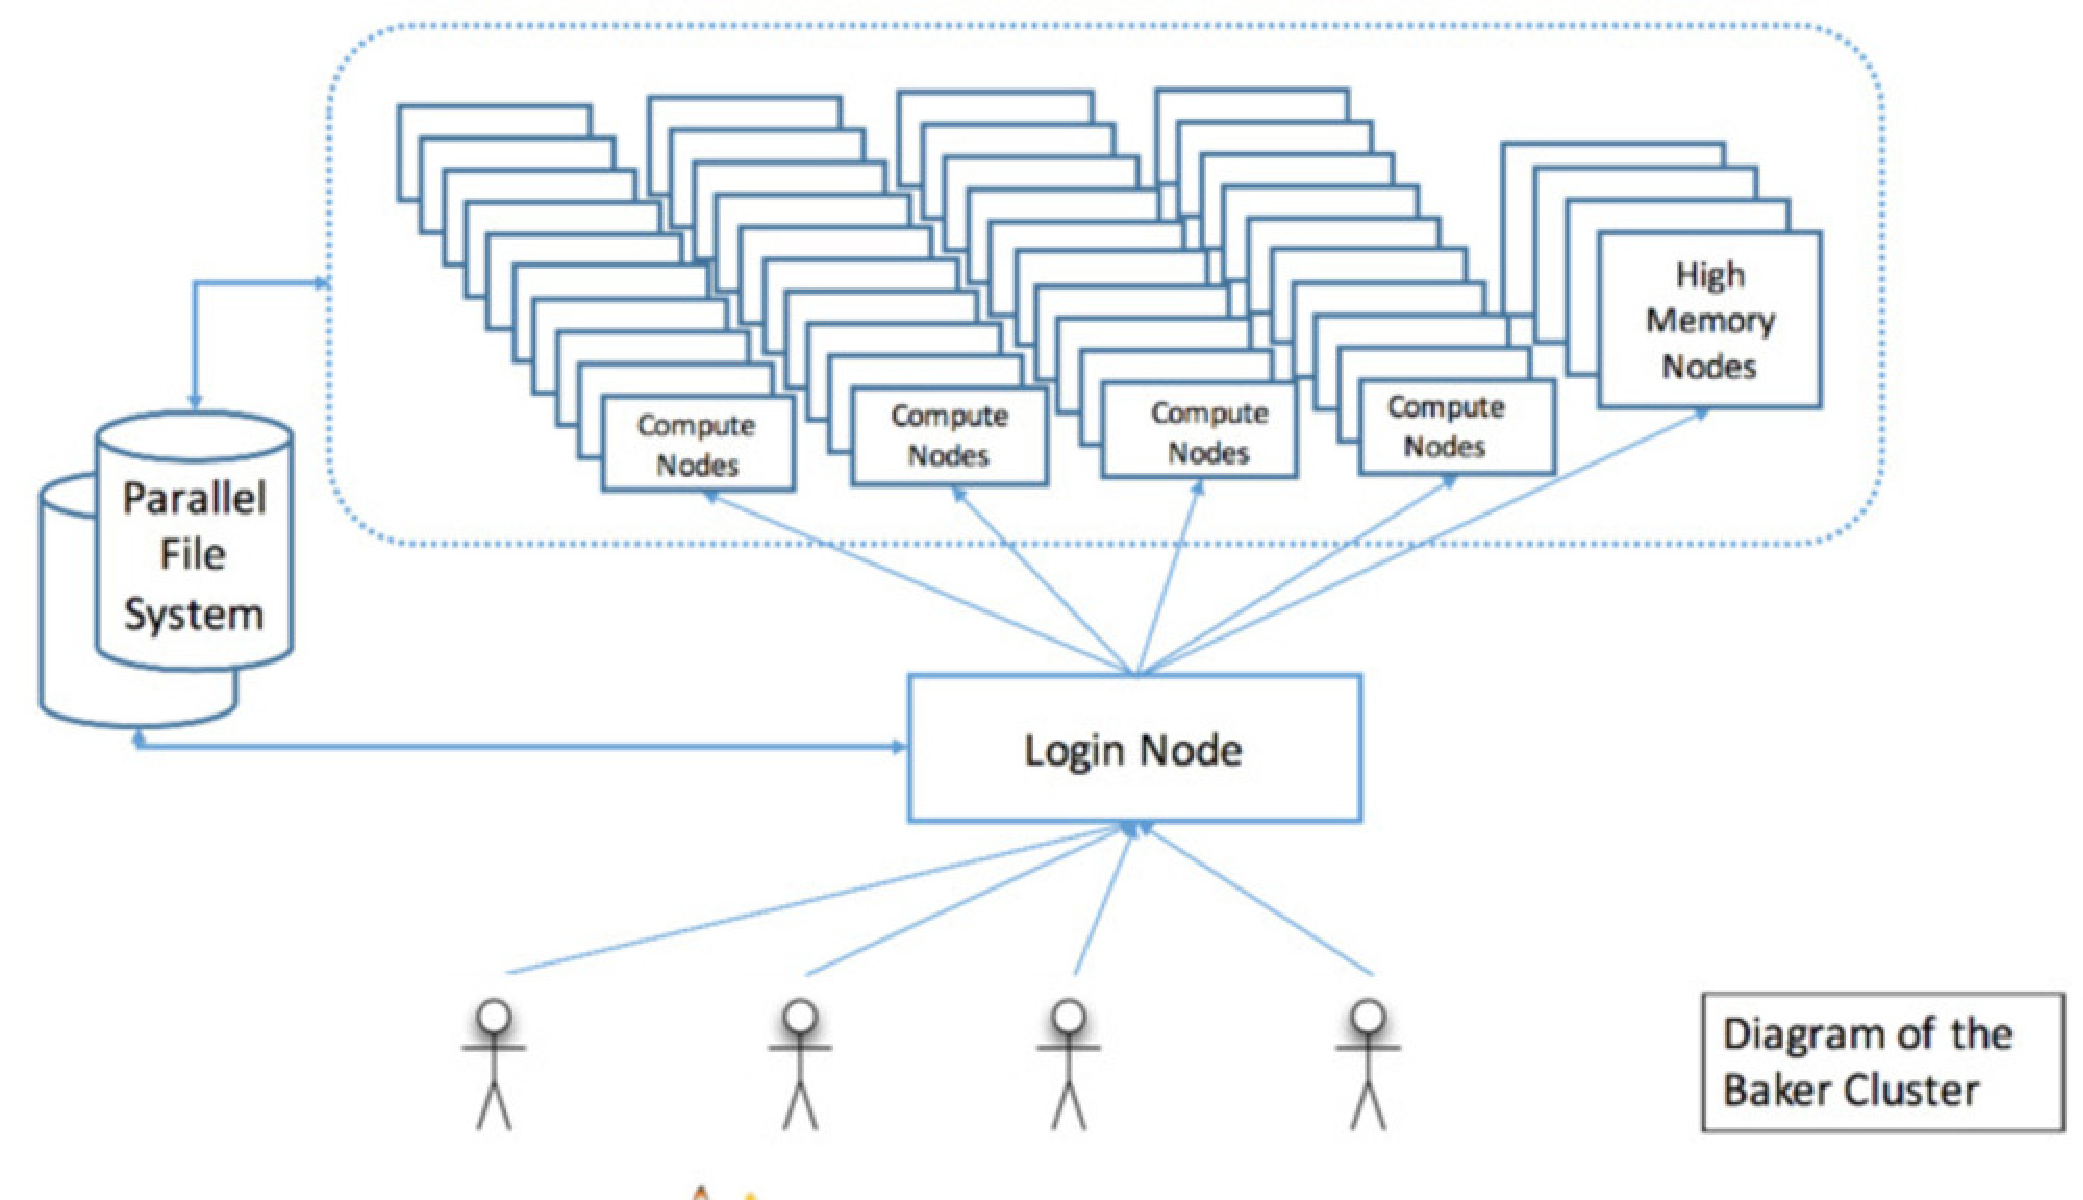
\includepdf{images/GPFS_File-eps-converted-to.pdf}
%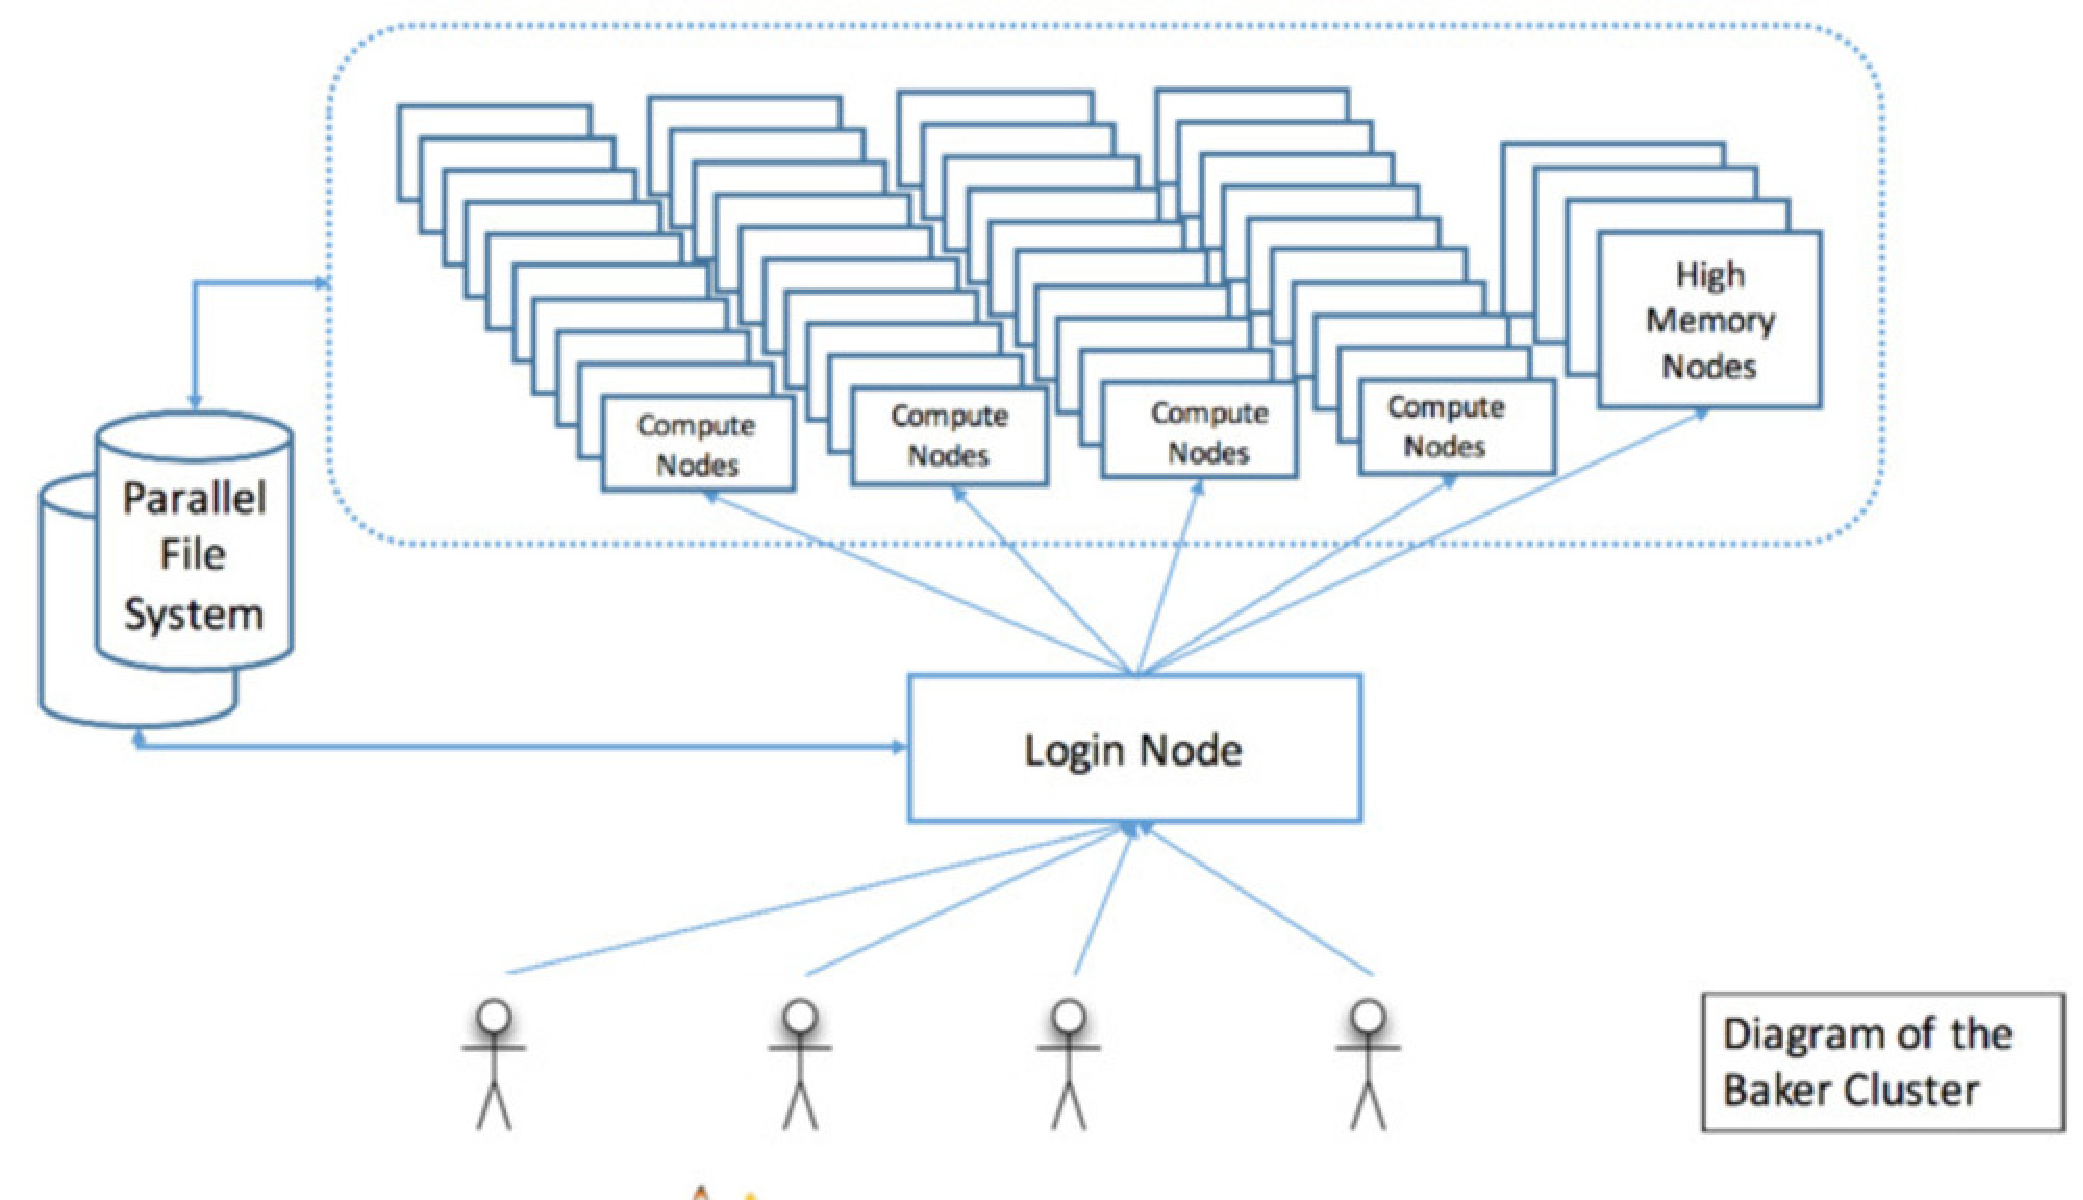
\includepdf{images/GPFS_File-eps-converted-to.pdf}

\put(0, 70){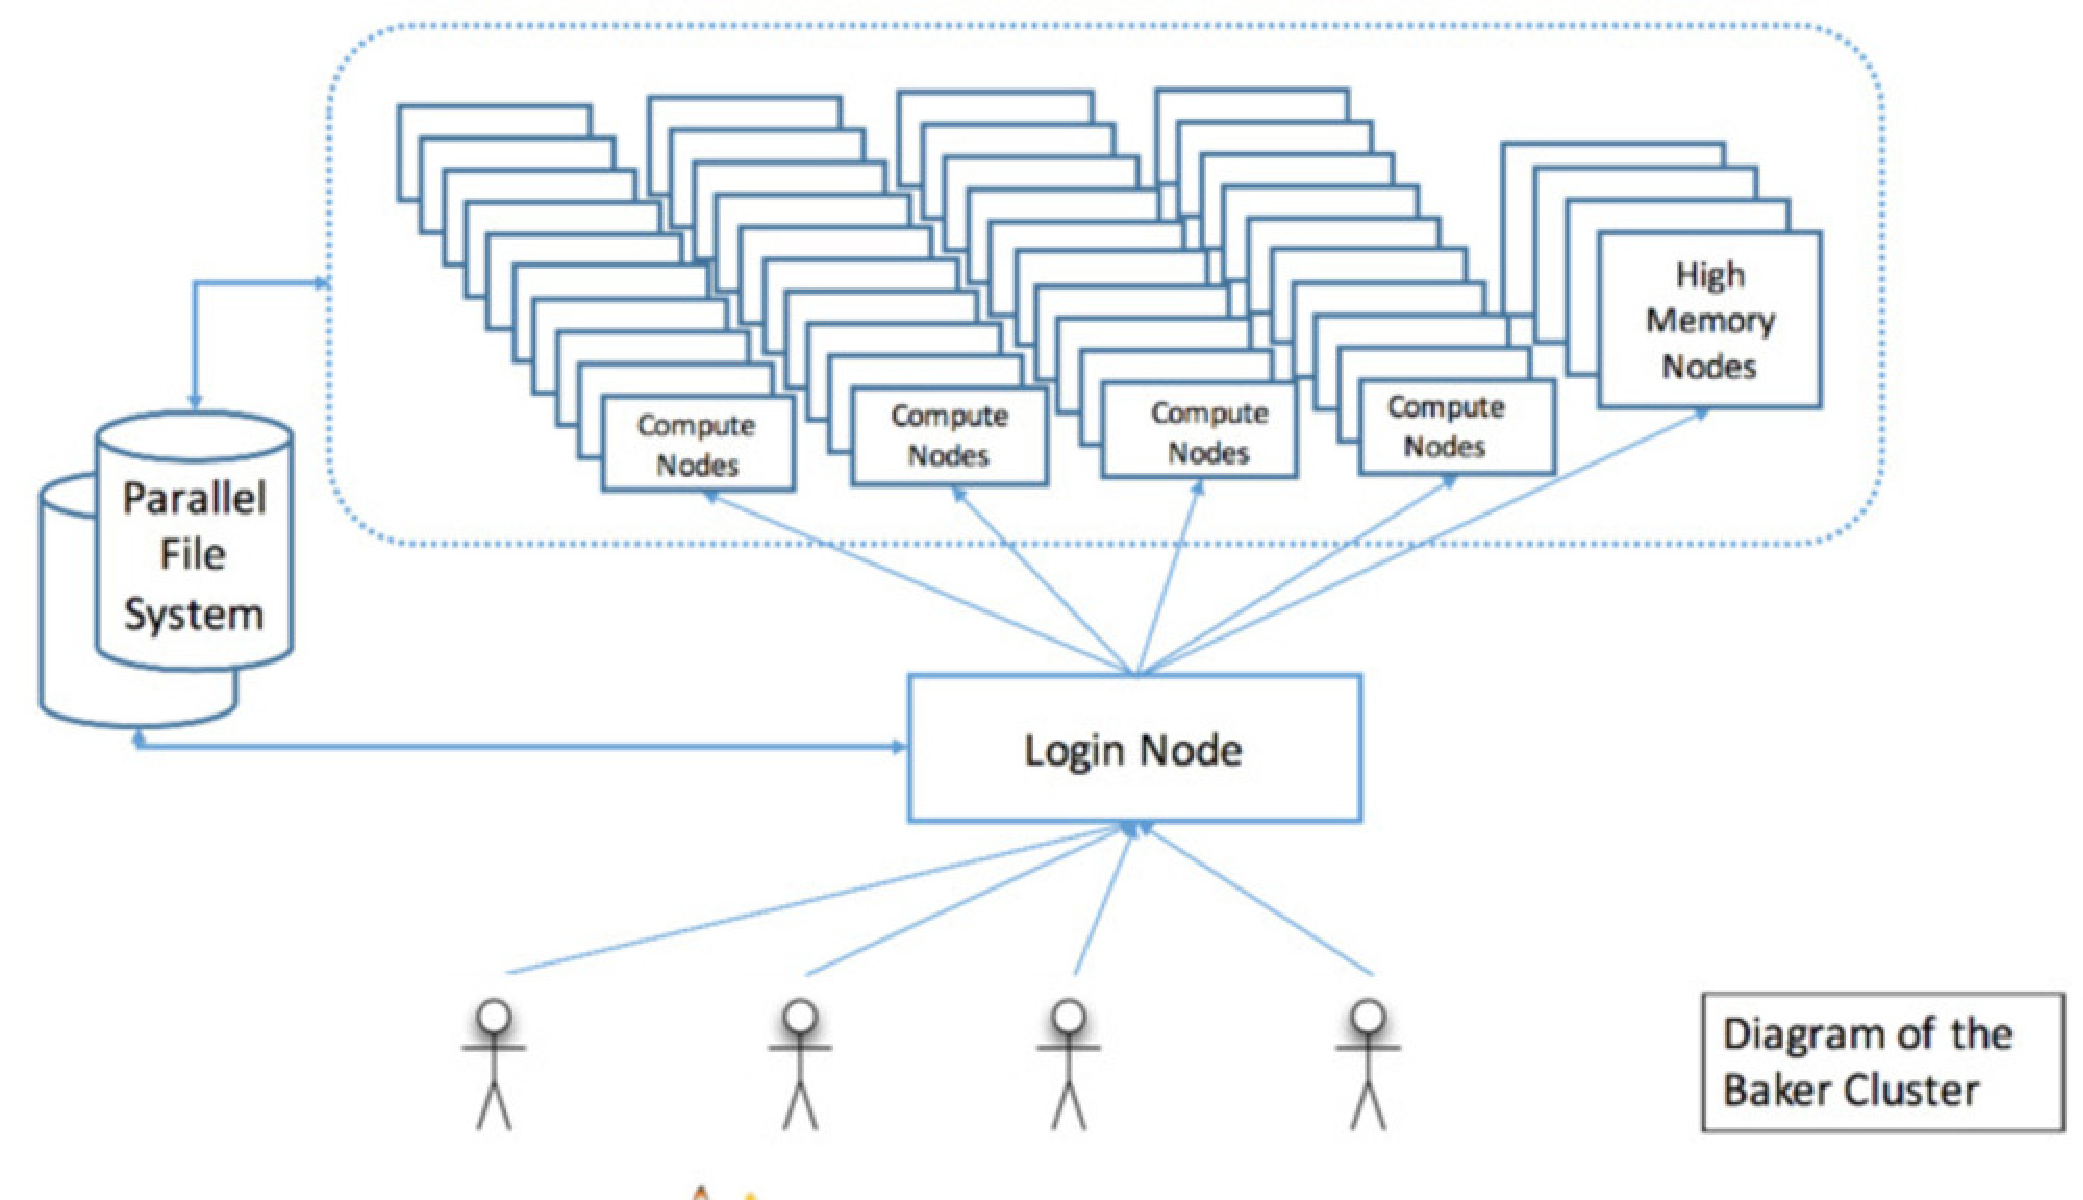
\includegraphics[height=2.5in]{images/GPFS_File-eps-converted-to.pdf}}
\end{picture}
\end{frame}



\begin{frame}
\frametitle{What is Linux?}
Operating System
\begin{itemize}
    \item Bootloader 
    \item Kernel - interface between the hardware and operating system. Manages processes.
    \item Daemons - background processes
    \item Graphical Interface -  X11 or X
    \item Shell - a.k.a. ``The Command Line".  This will be where you interface with Linux.
\end{itemize}
\end{frame}
 

\begin{frame}
\frametitle{Why use Linux?}
\begin{itemize}
    \item Package managers (e.g. \code{yum})
    \bigskip
    \item Built for programming. Comes with compilers, editors etc.
    \bigskip
    \item Great online resources (e.g. https://stackoverflow.com/)
    \bigskip
    \item Customizable
    \bigskip
    \item Dominant HPC platform.
\end{itemize}
\end{frame}
 

\begin{frame}
\frametitle{Types of Users}
\begin{itemize}
    \item Regular users (you)
    \bigskip

    \item Priveleged users (Yuan and myself)
    \bigskip

    \begin{itemize}
        \item Can modify \code{/usr}, \code{/opt}, etc.
        \bigskip

        \item \code{sudo}
    \end{itemize}
\end{itemize}
\end{frame}


\begin{frame}
\frametitle{The ``Shell"}
%\begin{picture}(320,250)  %must be related to where it is centered
%%\put(-30, 200){\includegraphics[height=0.8in]{images/Panoramic_Austin.jpg}}
%\put(100, 100){\includegraphics[height=1.8in]{images/shell.eps}}
%\end{picture}
%\begin{tabular}{cl}  
%  \begin{tabular}{c}
%    \includegraphics[height=7cm, width=4.5cm]{images/shell.eps}
%    \end{tabular}
%    & \begin{tabular}{l}
%      \parbox{0.5\linewidth}{%  change the parbox width as appropiate
    \begin{itemize}
        \item Used at the command line, i.e. the `terminal'
        \bigskip
        \item The user interface with the operating system
        \bigskip
        \item Bash is the default shell on Baker.
    \end{itemize}
%    }
%    \end{tabular}  \\
%\end{tabular}
\end{frame}


\begin{frame}
\frametitle{Text Editors}
\begin{itemize}
    \item \code{vim}   : Command line based
    \bigskip
    \item \code{emacs} : Command line based
    \bigskip
    \item \code{gedit} : Graphical  based
\end{itemize}
\end{frame}

%\begin{frame}
%\begin{picture}(320,250)  %must be related to where it is centered
%\put(20, 10){\includegraphics[height=3.5in, width=3.5in]{images/vim.eps}}
%\end{picture}
%\frametitle{Vim}
%\end{frame}

\begin{frame}
\frametitle{Basic Commands}
\code{vim} - text editor
\bigskip
\begin{itemize}
    \item \code{vim $\sim$/Scatch/tmp.txt}
    \bigskip
    \item Command and Edit modes.
    \bigskip
    \item \code{esc} to enter command mode
    \bigskip
    \item \code{i} to enter edit mode
    \bigskip
    \item To save, in command mode : \code{esc} \code{:w}
    \bigskip
    \item To quit, in command mode : \code{esc} \code{:q}
\end{itemize}
\end{frame}

\begin{frame}
\frametitle{Basic Commands}
\code{ls} - List directories and files. E.g.
\bigskip
\begin{itemize}
    \item \code{ls /opt/python }
    \bigskip

    \item \code{ls -l /opt/python} 
\end{itemize}
\end{frame}



\begin{frame}
\frametitle{Basic Commands}
\code{mkdir} - Make directories. E.g.
\bigskip
\begin{itemize}
    \item \code{mkdir $\sim$/Scratch/newdir}
\end{itemize}
\end{frame}


\begin{frame}
\frametitle{Basic Commands}
\code{man} - prints user manual for command. E.g.
\bigskip
\begin{itemize}
    \item \code{man ls}
    \bigskip
    \item Use \code{d} and \code{b} to navigate forward and back.
    \bigskip
    \item Use \code{q} to quit
    \bigskip
    \item Use \code{/somestring} to search for \code{somestring} within the man page.
\end{itemize}
\end{frame}


\begin{frame}
\frametitle{Basic Commands}
\code{cd}- Change directory. E.g.
\bigskip
\begin{itemize}
    \item \code{cd $\sim$/Scratch}
    \bigskip
    \item \code{cd}
    \bigskip
    \item \code{cd ..}
    \bigskip
    \item \code{cd $\sim$} 
\end{itemize}
\end{frame}


\begin{frame}
\frametitle{Basic Commands}
\code{pwd}- print working directory. E.g.
\bigskip
\begin{itemize}
    \item \code{pwd}
\end{itemize}
\end{frame}


\begin{frame}
\frametitle{Basic Commands}
\code{touch}- Create empty file. E.g.
\bigskip
\begin{itemize}
    \item \code{touch $\sim$/Scratch/file.txt}
\end{itemize}
\end{frame}


\begin{frame}
\frametitle{Basic Commands}
\code{mv}- move file or rename file. E.g.
\bigskip
\begin{itemize}
    \item \code{mv $\sim$/Scratch/file.txt $\sim$/Scratch/file2.txt}
\end{itemize}
\end{frame}

\begin{frame}
\frametitle{Basic Commands}
\code{cp}- copy files or directories
\bigskip
\begin{itemize}
    \item \code{cp $\sim$/Scratch/file.txt $\sim$/Scratch/file2.txt}
    \bigskip
    \item \code{cp -r $\sim$/Scratch/newdir $\sim$/Scratch/newdir2}
\end{itemize}
\end{frame}


\begin{frame}
\frametitle{Basic Commands}
\code{rm}- delete files or directories. Be Careful. E.g.
\bigskip
\begin{itemize}
    \item \code{rm $\sim$/Scratch/file.txt}
    \bigskip
    \item \code{rm -r $\sim$/Scratch/newdir}
\end{itemize}
\end{frame}


\begin{frame}
\frametitle{Basic Commands}
\code{cat}- concatenate files. E.g.
\bigskip
\begin{itemize}
    \item \code{cat /opt/modulefiles/gcc-4.9.2}
\end{itemize}
\end{frame}


\begin{frame}
\frametitle{Basic Commands}
\code{echo}- echo back string. E.g.
\bigskip
\begin{itemize}
    \item \code{echo "Hello World"}
\end{itemize}
\end{frame}


\begin{frame}
\frametitle{Permissions}
\code{chmod}- Change permissions.
E.g.
\begin{itemize}
    \item \code{ls -l $\sim$/Scratch/file.txt}, yields : 
    \hspace{5mm} \code{-rw-r--r--  1 user group 0 Apr  5 09:01 file.txt}
    \smallskip
\end{itemize}
\bigskip


% http://www.texample.net/tikz/examples/beamer-arrows/
% https://tex.stackexchange.com/a/83434/84495

\begin{tikzpicture}[overlay]

%\coordinate (G) at (2.3,6.1);
\coordinate (A) at (1.15,1.3);
\coordinate (AU) at (1.15,1.5);
\coordinate (B) at (1.65,1.3);
\coordinate (BU) at (1.8,1.5);
%\coordinate (AB1) at (1.35,1.3);
\coordinate (AB1) at (1.55,1.3);
\coordinate (AB2) at (0.5,0.3);


\coordinate (C) at (1.80,1.3);
\coordinate (D) at (2.35,1.3);
\coordinate (CD1) at (2.15,1.3);
\coordinate (CD2) at (2.15,0.3);


\coordinate (E) at (2.50,1.3);
\coordinate (EU) at (2.50,1.5);
\coordinate (F) at (3.0,1.3);
\coordinate (F1) at (3.15,1.3);
\coordinate (FU) at (3.15,1.5);
\coordinate (EF1) at (2.75,1.3);
\coordinate (EF2) at (3.60,0.4);

\draw [red,<-<,ultra thick]    (A) to[out=0,in=0] (B);
\draw [red,-]    (A) -- (AU);
\draw [red,-]    (C) -- (BU);
\draw [red,-,ultra thick]    (AB1) -- (AB2);
\draw [blue,<-<,ultra thick]   (C) to[out=0,in=0] (D);
\draw [blue,-,ultra thick]   (CD1) -- (CD2);
\draw [black,<-<,ultra thick] (E) to[out=0,in=0] (F);
\draw [black,-]    (E) -- (EU);
\draw [black,-]    (F1) -- (FU);
\draw [black,-,ultra thick,bend right] (EF1) to[out=0,in=0] (EF2);
\node[draw,red] at (0,0) {you};
\node[draw,blue] at (2.15,-0) {group};
\node[draw,black] at (4.8, -0) {everyone else};
\draw [red,-,ultra thick]    (0.5,0) -- (2.25,-0.6);
\draw [blue,-,ultra thick]   (2.6,-0.25) -- (2.6,-0.6);
\draw [black,-,ultra thick]  (3.5,-0.250) -- (2.8,-0.6);
\end{tikzpicture}
\bigskip
\pause
\begin{itemize}
    \smallskip
    \item \code{chmod 755 file.txt}
    \pause
    \bigskip
    %\item \code{ls -l $\sim$/Scratch/file.txt}, yields : 
    %\hspace{5mm} \code{-rwxr-xr-x  1 user group 0 Apr  5 09:01 file.txt}
    \item {\small \code{-rwxr-xr-x  1 user group 0 Apr  5 09:01 file.txt}}
\end{itemize}
\pause

\bigskip
Explanation:
\begin{itemize}
    %\item First number is you.
    %\item Second number is for your group (i.e. lab).
    %\item Third number is for everyone else.
    \item \code{r} = 4, \code{w} = 2, \code{x} = 1
    \item \code{7} = \code{4} + \code{2} + \code{1} = read (\code{r}) + write (\code{w}) +  execute(\code{x})
    \item \code{5} = \code{4} + \code{1} = read (\code{r}), execute(\code{x})
\end{itemize}


\end{frame}



%\begin{frame}
%\frametitle{Permissions}
%\code{chmod}- Change permissions.
%E.g.
%\begin{itemize}
%    \item \code{ls -l $\sim$/Scratch/file.txt}, yields : 
%    \hspace{5mm} \code{-rw-r--r--  1 user group 0 Apr  5 09:01 file.txt}
%    \smallskip
%    \item \code{chmod 755 somescript.sh}
%    \bigskip
%    \item \code{ls -l $\sim$/Scratch/file.txt}, yields : 
%    \hspace{5mm} \code{-rwxr-xr-x  1 user group 0 Apr  5 09:01 file.txt}
%\end{itemize}
%\bigskip
%
%Explanation:
%\begin{itemize}
%    \item First number is you.
%    \item Second number is for your group (i.e. lab).
%    \item Third number is for everyone else.
%    \item \code{r} = 4, \code{w} = 2, \code{x} = 1
%    \item \code{7} = \code{4} + \code{2} + \code{1} = read (\code{r}) + write (\code{w}) +  execute(\code{x})
%    \item \code{5} = \code{4} + \code{1} = read (\code{r}), execute(\code{x})
%\end{itemize}
%\end{frame}
%


\begin{frame}
\frametitle{Homework}
Create a bash script that says ``Hello World". Make it executable. 

\bigskip

\emph{HINT}, you'll need to add $\code{\#^^21/bin/bash}$ at the top of your script
\end{frame}


\begin{frame}
\frametitle{References}
\begin{itemize}
    \item https://www.opensourceforu.com/2020/03/reasons-to-use-linux/
    \item https://www.extremetech.com/extreme/155392-international-space-station-switches-from-windows-to-linux-for-improved-reliability
    \item https://medium.com/geekculture/how-to-stop-windows-10-from-spying-on-you-b071134a11f6
    \item https://washingtonsblog.com/microsoft-programmed-in-nsa-backdoor-in-windows-by-1999/
    \item https://security.stackexchange.com/a/96715/94605
    \item https://medium.com/geekculture/how-linux-helped-us-land-on-mars-a2ceb54cf6e
    \item https://www.lbto.org/software-eng-202102.html
    \item https://www.skatelescope.org/software-and-computing/
\end{itemize}
\end{frame}

\end{document}





